%!TEX root = main.tex
\chapter{TRIAC en tryristor}
\label{TRIAC_en_tryristor}

\section{Tryristor}
Een tryristor heeft de volgende schakeling:

\begin{center}
    \begin{circuitikz}
        \draw (0,0) to [isourcesin](0,2)
        to [Ty, n=Tro](2,2)
        to [european resistor](2,0)
        to [short](0,0);
    \end{circuitikz}
\end{center}

Met het symbool $\alpha$ wordt de stuurhoek aangegeven. Dit is de hoek waar het signaal bij begint. het signaal voor deze hoek is
afgekapt en dus afwezig. Dit wordt elke $2\pi$ herhaald. Het stuk tussen 0 graden een de stuurhoek is dus altijd 0.

Over $U_R$ staat ook deze spanning. De spanning is echter alleen positief. De negative spanningen zijn over de weerstand 0v.

Bij het rekenen aan de schakeling horen de volgende formules:

$U_{Rrms}=\frac{\hat{u}}{2}\sqrt{\frac{\pi -\alpha }{\pi }+\frac{\sin (2\alpha )}{2\pi }}$

$U_{1rms}=\frac{\sqrt{a_1^2 + b_1^2}}{2\pi }$

$a_1=\frac{\hat{u}}{2 \pi} \left(\pi - \alpha + \frac{\sin (2 \alpha)}{2}\right) $

$b_1=\frac{\hat{u}}{2 \pi} \left(\frac{\cos (2 \alpha)}{2} \right) $

$S_1=U_b \cdot I_1$

$I_1=\frac{U_b}{R}$

\vspace{5mm}

De rest van de formules zijn makkelijk te achter halen met behulp van de vermogens driehoek. Deze kan voor de berekeningen van de 
tryristor en de TRIAC worden uitgebreid. Dit komt er dan als volgende uit te zien:

\begin{center}

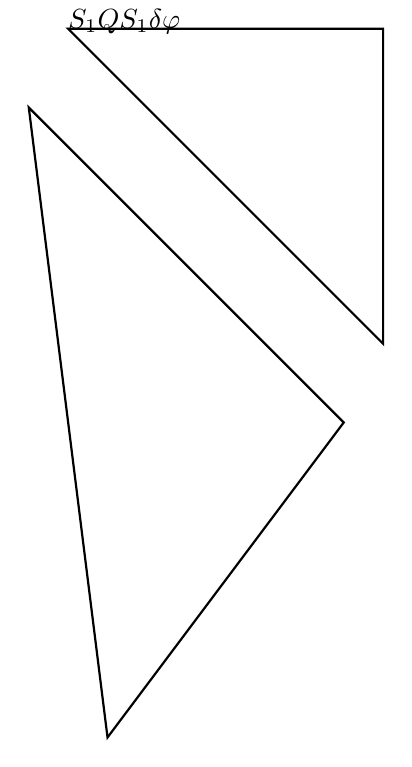
\begin{tikzpicture}[thick]
\coordinate (O) at (0,0);
\coordinate (A) at (4,0);
\coordinate (B) at (4,-4);
\draw (O)--(A)--(B)--cycle;

\coordinate (x) at (3.5,-5);
\coordinate (y) at (-0.5,-1);
\coordinate (z) at (0.5,-9);
\draw (x)--(y)--(z)--cycle;

\tkzLabelSegment[above=2pt](O,A){\textit{P}}
\tkzLabelSegment[left=2pt](O,B){\textit{$S_1$}}
\tkzLabelSegment[above right=0pt](A,B){\textit{$Q$}}

\tkzLabelSegment[left=2pt](y,z){\textit{S}}
\tkzLabelSegment[left=2pt](x,y){\textit{$S_1$}}
\tkzLabelSegment[below=2pt](x,z){\textit{D}}

\tkzMarkAngle[fill= teal,size=0.8cm,%
opacity=.4](B,O,A)
\tkzLabelAngle[pos = -0.6](A,O,B){$\delta $}

\tkzMarkAngle[fill= teal,size=0.8cm,%
opacity=.4](z,y,x)
\tkzLabelAngle[pos = -0.6](x,y,z){$\varphi $}

\end{tikzpicture}
\end{center}

binnen de driehoek geldt: 

$S_1=$ Eerste harmonische van S

$S=$ Totaal vermogen.

$D=$ Distortie vermogen.

\section{TRIAC}
Een TRIAC heeft net een andere, maar vergelijkbare schakeling:
\begin{center}
    \begin{circuitikz}
        \draw (0,0) to [isourcesin](0,2)
        to [Tr, n=Tyo](2,2)
        to [european resistor](2,0)
        to [short](0,0);
    \end{circuitikz}
\end{center}

Voor de TRIAC gelden de zelfde formules er, maar omdat de schakeling anders is zijn er wel 3 formules verandert:

$U_{Rrms}=\frac{\hat{u}}{\sqrt{2}}\sqrt{\frac{\pi -\alpha }{\pi }+\frac{\sin (2\alpha )}{2\pi }}$

$a_1=2\frac{\hat{u}}{2 \pi} \left(\pi - \alpha + \frac{\sin (2 \alpha)}{2}\right) $

$b_1=2\frac{\hat{u}}{2 \pi} \left(\frac{\cos (2 \alpha)}{2} \right)$